%% ============================================================================
%%  Project 3 report: 5-Stage Pipelined RISC-V Processor
%%  IEEE conference format (IEEEtran). Build:  tectonic report.tex
%%  Figures in figures/ are generated from the simulation output by
%%  scripts/model.py and scripts/figures.py (see Appendix A).
%%  Build from this folder:  tectonic report.tex
%% ============================================================================
\documentclass[conference]{IEEEtran}

\usepackage[T1]{fontenc}
\usepackage{amsmath,amssymb}
\usepackage{graphicx}
\usepackage{booktabs}
\usepackage{multirow}
\usepackage{array}
\newcolumntype{L}[1]{>{\raggedright\arraybackslash}p{#1}}
\usepackage{xcolor}
\usepackage{tikz}
\usetikzlibrary{arrows.meta,positioning,calc,fit,shapes.geometric}
\usepackage{cite}
\usepackage[hidelinks]{hyperref}
\usepackage{url}
\usepackage{balance}

%% ---- Edit these before submission ------------------------------------------
\newcommand{\institution}{Rishihood University}
\newcommand{\course}{Modern Computer Architecture, B.Tech (CS\&AI)}
\newcommand{\instructor}{Sujit Kumar}
\newcommand{\repourl}{https://github.com/WhiteHacker000/RISC-V-PIPELINE}
%% ----------------------------------------------------------------------------

\definecolor{accent}{HTML}{2A78D6}
\definecolor{warm}{HTML}{EB6834}
\definecolor{ink}{HTML}{1F1F1E}
\definecolor{muted}{HTML}{8A8A83}
\definecolor{regfill}{HTML}{E8EEF7}
\definecolor{unitfill}{HTML}{F6F6F3}
\definecolor{hazfill}{HTML}{FDEDE6}

\newcommand{\code}[1]{\texttt{\small #1}}
\newcommand{\yes}{\textcolor{accent}{\textbf{1}}}
\newcommand{\no}{\textcolor{muted}{0}}

\begin{document}

\title{Design, Verification and Performance Analysis of a\\Five-Stage Pipelined RISC-V Processor}

\author{
\IEEEauthorblockN{%
\begin{tabular}{@{}ccccc@{}}
Nishant Sharma & Kushal Tyagi & Dev Tyagi & Vansh Khod & Anant Lalwani \\[-1pt]
{\normalsize\itshape 2401010302} & {\normalsize\itshape 2401010249} & {\normalsize\itshape 2401010148} & {\normalsize\itshape 2401010493} & {\normalsize\itshape 2401020086}
\end{tabular}}
\IEEEauthorblockA{\course\\
\institution\\
Project 3 \quad$\cdot$\quad Instructor: \instructor\\
Source: \url{\repourl}}
}

\maketitle

%% ============================================================================
\begin{abstract}
We present a five-stage (IF--ID--EX--MEM--WB) pipelined processor for a seven-instruction subset of RV32I (ADD, SUB, ADDI, LW, SW, BEQ, BNE), written as modular, synthesisable SystemVerilog. The core resolves data hazards with EX/MEM and MEM/WB forwarding plus a write-back-to-decode bypass, interlocks for one cycle on a load-use dependency, and resolves branches in EX with a two-instruction flush. Every module has a self-checking testbench. Two integration benches run complete programs and check the pipeline invariants on every clock cycle. Mutation testing shows that the final suite detects 14 of 14 injected hazard, flush and reset bugs, whereas the original integration test detected 3. Hardware performance counters give a CPI of 1.67--2.33 on five short benchmarks and 1.06 on a 64-instruction stream. The cycle count equals $N+4+\text{stalls}+2\times\text{taken branches}$ exactly in every case. An issue-timing model, validated against those counters, shows that forwarding saves up to 36\% of cycles over a stall-only design. Yosys synthesis for a Xilinx 7-series device uses about 469 LUTs and 349 flip-flops. Maximum clock frequency was not measured; Section~\ref{sec:synth} explains why and how to obtain it.
\end{abstract}

\begin{IEEEkeywords}
RISC-V, pipelining, data hazards, forwarding, load-use stall, branch flush, CPI, verification, mutation testing, SystemVerilog, FPGA synthesis.
\end{IEEEkeywords}

%% ============================================================================
\section{Introduction}

A single-cycle processor finishes each instruction in one long clock cycle. That cycle must cover instruction fetch, register read, ALU, data memory and write-back in series. Pipelining splits this path into stages separated by registers, so that one instruction can enter each stage per cycle. In the ideal case this gives a CPI (cycles per instruction) of one at a much shorter clock period~\cite{patterson-riscv,hennessy-quant}. In practice, instructions in flight depend on one another, and the hardware must detect and resolve these \emph{hazards} without changing the program's result.

The objective of Project~3 is to design a five-stage pipelined RISC-V processor and study the effect of pipelining on execution performance. This report describes:
\begin{itemize}
  \item the datapath, its four pipeline registers, and the control for a seven-instruction RV32I subset (Sections~\ref{sec:arch}--\ref{sec:impl});
  \item the hazard logic: forwarding, a WB$\rightarrow$ID bypass, load-use interlock and branch flush, with an explicit priority order (Section~\ref{sec:hazards});
  \item the verification: unit and integration benches, cycle-level invariant checking, and mutation testing that measures how good the tests are (Section~\ref{sec:verif});
  \item measured CPI and IPC, an exact cycle-count model, and comparisons with a stall-only baseline, a stall-on-branch baseline and a single-cycle design (Section~\ref{sec:perf});
  \item synthesis resource results and their limits (Section~\ref{sec:synth}).
\end{itemize}
Table~\ref{tab:compliance} maps each project requirement to where it is addressed.

\begin{table}[t]
\centering
\caption{Project requirements and where they are addressed}
\label{tab:compliance}
\footnotesize
\begin{tabular}{@{}L{3.55cm}L{1.15cm}p{2.6cm}@{}}
\toprule
Requirement & Section & Status \\
\midrule
Block diagram and explanation & \ref{sec:arch} & Fig.~\ref{fig:datapath} \\
Microarchitecture description & \ref{sec:arch}, \ref{sec:hazards} & Tables~\ref{tab:control}--\ref{tab:hazards} \\
Synthesisable modular RTL & \ref{sec:impl} & 15 modules \\
Dedicated testbenches & \ref{sec:verif} & 16 benches, all pass \\
Waveform verification & \ref{sec:verif-wave} & Figs.~\ref{fig:wave-lu}, \ref{fig:wave-br} \\
Pipeline registers, overlap, ordering & \ref{sec:verif}, \ref{sec:perf} & Fig.~\ref{fig:occ} \\
Dependent instruction sequences & \ref{sec:verif}, \ref{sec:perf} & 10-deep chain \\
Benchmark programs; CPI/IPC & \ref{sec:perf} & Table~\ref{tab:perf} \\
Comparison with a baseline & \ref{sec:perf-cmp} & Table~\ref{tab:policy} \\
Synthesis resource utilisation & \ref{sec:synth} & Table~\ref{tab:synth} \\
Maximum operating frequency & \ref{sec:synth} & \textbf{not measured} \\
FPGA deployment & \ref{sec:synth} & not done \\
\bottomrule
\end{tabular}
\end{table}

%% ============================================================================
\section{Architecture}
\label{sec:arch}

\subsection{Instruction subset}
The core implements the seven instructions in Table~\ref{tab:isa}, with encodings as defined in the RISC-V unprivileged specification~\cite{riscv-spec}. This subset is deliberately small. It still contains one of each pipeline-relevant behaviour: a register--register ALU operation, an immediate ALU operation, a load (the source of load-use hazards), a store, and two conditional branches (the source of control hazards). Exceptions, interrupts, byte and halfword accesses, and the other RV32I instructions are out of scope.

\begin{table}[t]
\centering
\caption{Supported RV32I subset}
\label{tab:isa}
\footnotesize
\begin{tabular}{@{}llccl@{}}
\toprule
Instr. & Fmt & opcode & f3 / f7 & Operation \\
\midrule
ADD  & R & \code{0110011} & 000 / 00 & $rd \leftarrow rs1 + rs2$ \\
SUB  & R & \code{0110011} & 000 / 20 & $rd \leftarrow rs1 - rs2$ \\
ADDI & I & \code{0010011} & 000      & $rd \leftarrow rs1 + \mathrm{imm}$ \\
LW   & I & \code{0000011} & 010      & $rd \leftarrow M[rs1 + \mathrm{imm}]$ \\
SW   & S & \code{0100011} & 010      & $M[rs1 + \mathrm{imm}] \leftarrow rs2$ \\
BEQ  & B & \code{1100011} & 000      & if $rs1 = rs2$: $pc \leftarrow pc + \mathrm{imm}$ \\
BNE  & B & \code{1100011} & 001      & if $rs1 \neq rs2$: $pc \leftarrow pc + \mathrm{imm}$ \\
\bottomrule
\end{tabular}
\end{table}

\subsection{Datapath}
Fig.~\ref{fig:datapath} shows the integrated datapath (\code{rtl/riscv\_top.sv}). Instruction and data memories are separate arrays of 256 words each (Harvard organisation), so a fetch and a data access never compete for one port.

\begin{figure*}[t]
\centering
\resizebox{\textwidth}{!}{%
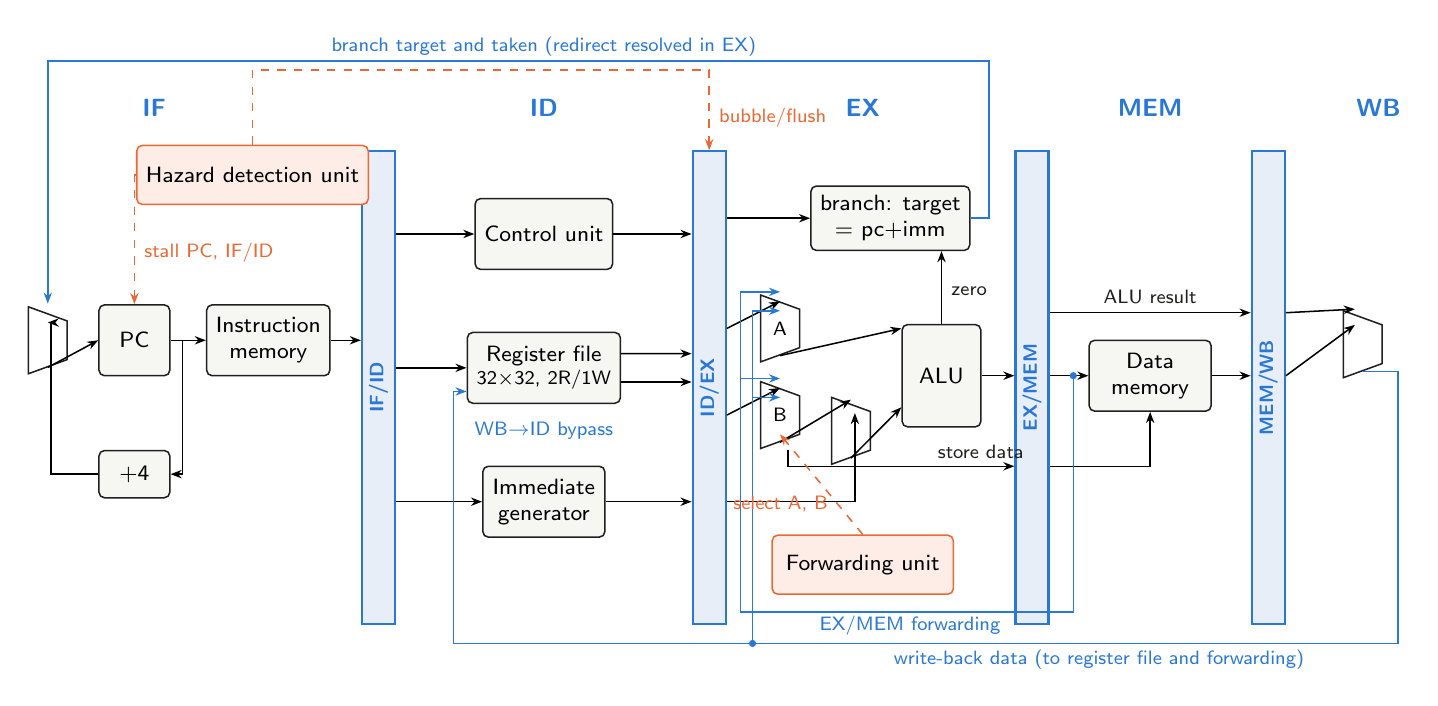
\begin{tikzpicture}[
  font=\sffamily\footnotesize, >={Stealth[length=4pt]}, line width=0.55pt,
  blk/.style={draw=ink, fill=unitfill, rounded corners=2pt, minimum width=1.55cm, minimum height=0.9cm, align=center},
  preg/.style={draw=accent, fill=regfill, line width=0.8pt, minimum width=0.42cm, minimum height=6.0cm},
  haz/.style={draw=warm, fill=hazfill, rounded corners=2pt, minimum width=2.3cm, minimum height=0.75cm, align=center},
  mux/.style={draw=ink, fill=white, trapezium, trapezium angle=70, shape border rotate=270, minimum width=0.85cm, minimum height=0.32cm, inner sep=1pt, font=\sffamily\scriptsize},
  stg/.style={font=\sffamily\bfseries\small, text=accent},
  lbl/.style={font=\sffamily\scriptsize, text=ink},
  fb/.style={->, draw=accent},
  hz/.style={->, draw=warm, dashed}
]
%% stage titles
\node[stg] at (1.6,3.55) {IF};
\node[stg] at (6.55,3.55) {ID};
\node[stg] at (10.6,3.55) {EX};
\node[stg] at (14.25,3.55) {MEM};
\node[stg] at (17.15,3.55) {WB};

%% pipeline registers
\node[preg] (ifid)  at (4.45,0) {}; \node[lbl, rotate=90, text=accent] at (4.45,0) {\textbf{IF/ID}};
\node[preg] (idex)  at (8.65,0) {}; \node[lbl, rotate=90, text=accent] at (8.65,0) {\textbf{ID/EX}};
\node[preg] (exmem) at (12.75,0) {}; \node[lbl, rotate=90, text=accent] at (12.75,0) {\textbf{EX/MEM}};
\node[preg] (memwb) at (15.75,0) {}; \node[lbl, rotate=90, text=accent] at (15.75,0) {\textbf{MEM/WB}};

%% IF
\node[mux] (pcmux) at (0.25,0.6) {};
\node[blk, minimum width=0.9cm] (pc) at (1.35,0.6) {PC};
\node[blk] (imem) at (3.05,0.6) {Instruction\\memory};
\node[blk, minimum width=0.9cm, minimum height=0.6cm] (add4) at (1.35,-1.1) {+4};
\draw[->] (pcmux.south) -- (pc.west);
\draw[->] (pc.east) -- (imem.west);
\draw[->] ($(pc.east)+(0.15,0)$) |- (add4.east);
\draw[->] (add4.west) -- ++(-0.6,0) |- ($(pcmux.north)+(0,-0.12)$);
\draw[->] (imem.east) -- ($(ifid.west)+(0,0.6)$);

%% ID
\node[blk] (ctrl) at (6.55,1.95) {Control unit};
\node[blk] (rf)   at (6.55,0.25) {Register file\\[-1pt]{\scriptsize 32$\times$32, 2R/1W}};
\node[blk] (imm)  at (6.55,-1.45) {Immediate\\generator};
\draw[->] ($(ifid.east)+(0,1.95)$) -- (ctrl.west);
\draw[->] ($(ifid.east)+(0,0.25)$) -- (rf.west);
\draw[->] ($(ifid.east)+(0,-1.45)$) -- (imm.west);
\draw[->] (ctrl.east) -- ($(idex.west)+(0,1.95)$);
\draw[->] ($(rf.east)+(0,0.18)$) -- ($(idex.west)+(0,0.43)$);
\draw[->] ($(rf.east)+(0,-0.18)$) -- ($(idex.west)+(0,0.07)$);
\draw[->] (imm.east) -- ($(idex.west)+(0,-1.45)$);
\node[lbl, text=accent, align=center] at (6.55,-0.55) {\scriptsize WB$\rightarrow$ID bypass};

%% EX
\node[mux] (fa) at (9.55,0.75) {A};
\node[mux] (fb) at (9.55,-0.35) {B};
\node[mux] (asrc) at (10.45,-0.55) {};
\node[blk, minimum width=1.0cm, minimum height=1.3cm] (alu) at (11.6,0.15) {ALU};
\node[blk, minimum width=1.55cm, minimum height=0.8cm] (br) at (10.95,2.15) {branch: target\\$=$ pc$+$imm};
\draw[->] ($(idex.east)+(0,0.75)$) -- (fa.north);
\draw[->] ($(idex.east)+(0,-0.35)$) -- (fb.north);
\draw[->] (fb.south) -- ($(asrc.north)+(0,0.05)$);
\draw[->] ($(idex.east)+(0,-1.45)$) -| ($(asrc.north)+(0.05,-0.12)$) ;
\draw[->] (fa.south) -- ($(alu.west)+(0,0.6)$);
\draw[->] (asrc.south) -- ($(alu.west)+(0,-0.4)$);
\draw[->] ($(idex.east)+(0,2.15)$) -- (br.west);
\draw[->] (alu.east) -- ($(exmem.west)+(0,0.15)$);
\draw[->] ($(fb.south)+(0.1,-0.1)$) |- ($(exmem.west)+(0,-1.0)$);
\node[lbl] at (12.1,-0.82) {\scriptsize store data};
\draw[->] (alu.north) -- (alu.north |- br.south) node[pos=0.45, right, lbl] {\scriptsize zero};

%% MEM
\node[blk] (dmem) at (14.25,0.15) {Data\\memory};
\draw[->] ($(exmem.east)+(0,0.15)$) -- (dmem.west);
\draw[->] ($(exmem.east)+(0,-1.0)$) -| (dmem.south);
\draw[->] (dmem.east) -- ($(memwb.west)+(0,0.15)$);
\draw[->] ($(exmem.east)+(0,0.95)$) -- ($(memwb.west)+(0,0.95)$);
\node[lbl] at (14.25,1.15) {\scriptsize ALU result};

%% WB
\node[mux] (wbmux) at (16.95,0.55) {};
\draw[->] ($(memwb.east)+(0,0.95)$) -- ($(wbmux.north)+(-0.1,0.1)$);
\draw[->] ($(memwb.east)+(0,0.15)$) -- ($(wbmux.north)+(-0.1,-0.1)$);

%% feedback: write-back to register file and forwarding
\draw[fb] (wbmux.south) -- ++(0.45,0) |- (5.4,-3.25) |- ($(rf.west)+(0,-0.3)$);
\draw[fb] (9.2,-3.25) |- ($(fa.north)+(0,-0.12)$);
\draw[fb] (9.2,-3.25) -- (9.2,-3.25) |- ($(fb.north)+(0,-0.12)$);
\fill[accent] (9.2,-3.25) circle (1.3pt);
\node[lbl, text=accent] at (13.6,-3.45) {write-back data (to register file and forwarding)};
%% EX/MEM forwarding
\draw[fb] ($(exmem.east)+(0,0.15)$) ++(0.3,0) |- (9.05,-2.85) |- ($(fa.north)+(0,0.12)$);
\draw[fb] (9.05,-2.0) |- ($(fb.north)+(0,0.12)$);
\fill[accent] ($(exmem.east)+(0.3,0.15)$) circle (1.3pt);
\node[lbl, text=accent] at (11.2,-3.03) {EX/MEM forwarding};

%% branch redirect to PC mux
\draw[fb] (br.east) -- (12.2,2.15) |- (0.25,4.15) -- ($(pcmux.north)+(0,0.12)$);
\node[lbl, text=accent] at (6.55,4.33) {branch target and taken (redirect resolved in EX)};

%% hazard units
\node[haz] (fwdu) at (10.6,-2.25) {Forwarding unit};
\node[haz] (hdu)  at (2.85,2.7) {Hazard detection unit};
\draw[hz] (fwdu.north) -- ($(fa.south)+(0,-1.0)$) node[pos=0.3, left, lbl, text=warm] {\scriptsize select A, B};
\draw[hz] (hdu.west) -| node[pos=0.8, right, lbl, text=warm] {stall PC, IF/ID} (pc.north);
\draw[hz] (hdu.north) -- ++(0,0.95) -| node[pos=0.8, right, lbl, text=warm] {bubble/flush} ($(idex.north)$);
\end{tikzpicture}}
\caption{Datapath of the five-stage core. The pipeline registers are shown in blue. Forwarding and write-back paths are blue arrows, and hazard-control signals are dashed orange. The register file is written at the clock edge that ends WB. A bypass in ID passes the value being written back to the instruction in decode, so that instruction sees it in the same cycle. A taken branch flushes IF/ID directly.}
\label{fig:datapath}
\end{figure*}

\subsection{Stages}
\textbf{IF:} the PC addresses instruction memory, which is read asynchronously. The next PC is PC$+4$ unless the pipeline is stalled (PC held) or a taken branch redirects it.

\textbf{ID:} the control unit decodes the opcode and validates \code{funct3}/\code{funct7}. Unsupported encodings produce no side effects. The immediate generator builds the sign-extended I/S/B immediate, and both source registers are read.

\textbf{EX:} two forwarding multiplexers choose each ALU operand from the register value, EX/MEM or MEM/WB. A third multiplexer chooses the immediate for ADDI, LW and SW. For branches the ALU subtracts, and the zero flag decides BEQ (zero) or BNE (non-zero). A separate adder computes the target $pc+\mathrm{imm}$.

\textbf{MEM:} LW and SW access the word-addressed data memory. Writes are synchronous and gated by reset.

\textbf{WB:} a multiplexer selects the loaded word or the ALU result. The register file ignores writes to x0.

\subsection{Pipeline registers}
Table~\ref{tab:pregs} lists what each register carries. All four registers use a synchronous active-low reset, and \emph{flush} takes priority over \emph{stall}. Flushing IF/ID inserts the canonical NOP \code{addi x0,x0,0}. Flushing ID/EX clears all control bits, which produces a bubble with no side effects.

\begin{table}[t]
\centering
\caption{Pipeline register contents}
\label{tab:pregs}
\footnotesize
\begin{tabular}{@{}lL{4.65cm}c@{}}
\toprule
Register & Fields & Stall / flush \\
\midrule
IF/ID  & pc, pc$+4$, instruction & yes / yes \\
ID/EX  & pc, pc$+4$, rs1/rs2 values, rs1/rs2/rd indices, immediate, ALU control, RegWrite, MemRead, MemWrite, Branch, BNE, ALUSrc, MemToReg & -- / yes \\
EX/MEM & ALU result, store data, branch target/taken, rd, pc$+4$, MemRead, MemWrite, RegWrite, MemToReg & -- / -- \\
MEM/WB & load data, ALU result, rd, RegWrite, MemToReg & -- / -- \\
\bottomrule
\end{tabular}
\end{table}

\subsection{Control}
The main decoder produces the control word from the opcode. The control unit then gates it with an instruction-valid check on \code{funct3}/\code{funct7} (Table~\ref{tab:control}). Branches use the ALU in subtract mode, and the separate BNE bit inverts the taken condition.

\begin{table}[t]
\centering
\caption{Control signals generated in ID}
\label{tab:control}
\footnotesize
\setlength{\tabcolsep}{3.6pt}
\begin{tabular}{@{}lccccccc@{}}
\toprule
 & RegWr & MemRd & MemWr & Br & ASrc & M2R & ALU \\
\midrule
ADD  & \yes & \no & \no & \no & \no & \no & add \\
SUB  & \yes & \no & \no & \no & \no & \no & sub \\
ADDI & \yes & \no & \no & \no & \yes & \no & add \\
LW   & \yes & \yes & \no & \no & \yes & \yes & add \\
SW   & \no & \no & \yes & \no & \yes & \no & add \\
BEQ/BNE & \no & \no & \no & \yes & \no & \no & sub \\
\bottomrule
\end{tabular}
\end{table}

%% ============================================================================
\section{Hazard Handling}
\label{sec:hazards}

Table~\ref{tab:hazards} summarises the three hazard classes and their cost. The design follows the classic organisation in~\cite{patterson-riscv}, with two refinements: x0 is never treated as a producer, and stalls are raised only for source fields that the decoded instruction actually reads.

\begin{table}[t]
\centering
\caption{Hazards, detection and resolution}
\label{tab:hazards}
\footnotesize
\begin{tabular}{@{}L{1.35cm}L{2.75cm}L{2.35cm}c@{}}
\toprule
Hazard & Detected when & Resolution & Cost \\
\midrule
ALU RAW, distance 1--2 & EX/MEM or MEM/WB writes a source of the instruction in EX & forward into ALU operand & 0 \\
RAW, distance 3 & WB writes a source of the instruction in ID & WB$\rightarrow$ID bypass & 0 \\
Load-use & load in EX writes a source used by the instruction in ID & hold PC and IF/ID; bubble into ID/EX & 1 \\
Control & BEQ/BNE taken in EX & redirect PC; flush IF/ID and ID/EX & 2 \\
Structural & -- & separate I/D memories & 0 \\
\bottomrule
\end{tabular}
\end{table}

\subsection{Forwarding}
For the operand $rs \in \{rs1, rs2\}$ of the instruction in EX, the forwarding unit computes
\begin{align*}
f_{\text{EX/MEM}} &= \text{RegWr}_{\text{M}} \wedge \neg\text{MemRd}_{\text{M}} \wedge rd_{\text{M}}\neq 0 \wedge rd_{\text{M}} = rs,\\
f_{\text{MEM/WB}} &= \text{RegWr}_{\text{W}} \wedge rd_{\text{W}}\neq 0 \wedge rd_{\text{W}} = rs,
\end{align*}
and selects EX/MEM if $f_{\text{EX/MEM}}$ holds, otherwise MEM/WB if $f_{\text{MEM/WB}}$ holds, otherwise the register value. Checking EX/MEM first returns the \emph{newest} value when both stages write the same register. A load in EX/MEM is never forwarded, because its data does not exist until the end of MEM. The two operands are selected independently, so one can come from EX/MEM while the other comes from MEM/WB. The forwarded rs2 also supplies the store data, so SW is covered without extra logic.

\subsection{Write-back to decode bypass}
The register file is written on the clock edge, so the instruction in ID would read a stale value while its producer is in WB. A small bypass in ID substitutes the write-back data when $\text{RegWr}_{\text{W}} \wedge rd_{\text{W}} \neq 0 \wedge rd_{\text{W}} = rs$. This closes the distance-3 case without a stall.

\subsection{Load-use interlock}
If the instruction in EX is a load whose $rd \neq 0$ matches a source the instruction in ID \emph{uses}, the hazard unit holds the PC and IF/ID for one cycle and flushes ID/EX. One cycle later the load is in MEM/WB, and the dependent instruction receives the value through MEM/WB forwarding. The ``uses'' qualifiers matter. ADDI and LW do not read rs2, so a coincidental match in their rs2 field does not stall. SW is treated as reading rs2, which is correct but conservative (Section~\ref{sec:disc}).

\subsection{Branches}
Branches are resolved in EX, and the pipeline fetches sequentially in the meantime (static not-taken). When a branch is taken, the PC is redirected to the target, and the two younger instructions in IF/ID and ID/EX are flushed. A taken branch therefore costs two cycles, and a not-taken branch costs nothing. A redirect takes priority over a simultaneous stall request in the hazard unit. In the integrated core this combination cannot occur, because ID/EX cannot hold a load and a branch at the same time.

\subsection{Reset}
The PC has an asynchronous active-low reset, while the pipeline registers reset synchronously. Register-file and data-memory writes are additionally gated by \code{rst\_n}, so an instruction in flight cannot commit a write while reset is asserted.

%% ============================================================================
\section{Implementation}
\label{sec:impl}

The RTL consists of 15 SystemVerilog modules (about 930 lines; Table~\ref{tab:modules}). The flow uses only open-source tools: Verilator~5.054~\cite{verilator} for linting and cycle-accurate simulation, Yosys~0.71~\cite{yosys} for synthesis, and Python for checking the counter output. A top-level \code{Makefile} provides the \code{build}, \code{run}, \code{test}, \code{lint}, \code{synth} and \code{wave} targets. \code{make test} compiles and runs every testbench and stops at the first failure.

\begin{table}[t]
\centering
\caption{RTL modules (each \code{X} has a unit bench \code{X\_tb}; \code{riscv\_top} has two integration benches)}
\label{tab:modules}
\footnotesize
\begin{tabular}{@{}lL{3.15cm}r@{}}
\toprule
Module & Function & Lines \\
\midrule
\code{program\_counter}       & PC: async reset, stall, redirect & 19 \\
\code{instruction\_memory}    & 256-word ROM, NOP fill & 32 \\
\code{register\_file}         & 32$\times$32, 2 read / 1 write, x0 $=0$ & 32 \\
\code{main\_decoder}          & opcode $\rightarrow$ control word & 47 \\
\code{control\_unit}          & funct check, ALU control & 73 \\
\code{immediate\_generator}   & I/S/B immediates & 22 \\
\code{alu}                    & add, sub, and, or, xor, slt(u) & 23 \\
\code{data\_memory}           & 256-word RAM, word access & 43 \\
\code{forwarding\_unit}       & ALU operand source select & 24 \\
\code{hazard\_detection\_unit}& load-use stall, flush & 23 \\
\code{if\_id} / \code{id\_ex} & pipeline registers & 24 / 76 \\
\code{ex\_mem} / \code{mem\_wb} & pipeline registers & 52 / 32 \\
\code{riscv\_top}             & integration, bypass, counters & 407 \\
\midrule
Total & 15 modules & 929 \\
\bottomrule
\end{tabular}
\end{table}

Beside the datapath, \code{riscv\_top} keeps simulation-only performance counters. A validity bit follows each instruction through the four pipeline registers. It is cleared by a flush or a bubble and held during a stall. The counters record active cycles, retired instructions, load-use stall cycles, branch flushes, and taken and not-taken branches. Bubbles, flushed instructions and the NOP fill do not retire.

%% ============================================================================
\section{Verification}
\label{sec:verif}

\subsection{Strategy}
Verification is layered. Sixteen self-checking testbenches run under \code{make test}: one per module, plus two integration benches. A run passes only if every bench prints its pass line and exits normally, and on the current main branch all 16 pass. The integration benches load hand-checked programs from \code{programs/*.hex}, run them on the full core, and compare final register and memory state as well as cycle-level behaviour.

\code{processor\_tb} runs the six benchmark programs of Section~\ref{sec:perf}. It checks results, instruction overlap, in-order write-back, and the exact values of every performance counter. \code{pipeline\_corner\_tb} runs seven core instances in parallel, one per verification target. A \emph{pipeline invariant monitor} is attached to every instance and checks, on each falling clock edge:
\begin{itemize}
  \item after a taken branch, IF/ID holds the NOP and ID/EX is a bubble;
  \item during a load-use stall, PC and IF/ID are unchanged and ID/EX is a bubble;
  \item no operand is ever forwarded from x0;
  \item no register or memory write comes from a slot marked invalid;
  \item its own stall and flush counts equal the hardware counters.
\end{itemize}

\begin{table}[t]
\centering
\caption{Integration corner cases (all pass)}
\label{tab:corner}
\footnotesize
\begin{tabular}{@{}L{1.55cm}L{6.15cm}@{}}
\toprule
Area & Scenarios checked \\
\midrule
x0 & ADDI/LW/SUB to x0 discarded; register 0 checked every cycle; x0 never forwarded, bypassed or load-use stalled \\
Forwarding & EX/MEM beats MEM/WB on rs1, rs2 and both; mixed sources per operand; store data and base forwarded \\
Dependencies & 10-deep chain, each ADD reading distance-1 and distance-2 results; distance-3 via WB$\rightarrow$ID bypass \\
Load-use & stall on load base, rs2, store data, store base and branch operand; no false stalls (exactly 5 stalls expected and seen) \\
Branches & backward loop taken twice then not taken; operands forwarded into the comparison; wrong-path ALU op, store and branch all suppressed \\
Reset & cold reset state; async PC reset mid-cycle; reset with a store and a write-back in flight; restart matches a cold-start reference \\
\bottomrule
\end{tabular}
\end{table}

Table~\ref{tab:corner} lists the integration corner cases. The corner-case programs come from a small Python encoder, whose output was cross-checked against the hand-written benchmark programs.

\subsection{Mutation testing}
Passing tests only show that no bug was \emph{found}. To measure whether the tests can find bugs, the script \code{verification/mutation\_check.sh} injects one bug at a time into a temporary copy of the RTL and reruns both integration benches~\cite{demillo-mutation}. Table~\ref{tab:mutation} shows the result. The original integration bench detects 3 of the 14 mutants. The corner-case bench detects all 14, including bugs that leave final register values unchanged, such as a missing IF/ID flush or x0 being written and then overwritten.

\begin{table}[t]
\centering
\caption{Mutation testing: injected bugs detected}
\label{tab:mutation}
\footnotesize
\setlength{\tabcolsep}{4pt}
\begin{tabular}{@{}lL{3.9cm}cc@{}}
\toprule
ID & Injected bug & \code{processor} & \code{corner} \\
\midrule
M1  & EX/MEM forwards x0 (rs1)           & --   & \yes \\
M2  & MEM/WB beats EX/MEM on rs2          & --   & \yes \\
M3  & hazard unit ignores rs2             & --   & \yes \\
M4  & load to x0 stalls                   & --   & \yes \\
M5  & IF/ID not flushed on taken branch   & --   & \yes \\
M6  & ID/EX not flushed on taken branch   & \yes & \yes \\
M7  & register file writes x0            & --   & \yes \\
M8  & no WB$\rightarrow$ID bypass         & \yes & \yes \\
M9  & data memory writes during reset     & --   & \yes \\
M10 & register file writes during reset   & --   & \yes \\
M11 & no bubble on load-use stall         & \yes & \yes \\
M12 & SW store data not a hazard source   & --   & \yes \\
M13 & EX/MEM forwards x0 (rs2)            & --   & \yes \\
M14 & MEM/WB forwards x0 (rs1)            & --   & \yes \\
\midrule
\multicolumn{2}{@{}l}{Detected} & 3/14 & \textbf{14/14} \\
\bottomrule
\end{tabular}
\end{table}

\subsection{Initial-state robustness}
The register file has no reset, which RISC-V permits because only x0 has a defined value. Verilator initialises state to zero by default, which can hide a dependence on initial values. We therefore also ran both integration benches with random initialisation (\code{--x-initial unique}). \code{pipeline\_corner\_tb} passes on 8 random seeds. \code{processor\_tb} fails, because one of its checks expects two never-written registers to be zero. This is a testbench assumption, not an RTL defect. We documented it and left the check unchanged for its owner.

\subsection{Waveform evidence}
\label{sec:verif-wave}
Figs.~\ref{fig:wave-lu} and~\ref{fig:wave-br} are drawn directly from the VCD dump that \code{make test} produces. Fig.~\ref{fig:occ} reconstructs, from the same dump, which instruction occupies each stage in each cycle. The reconstruction script asserts that its result matches the PC values held in IF/ID, ID/EX and EX/MEM in every cycle.

\begin{figure*}[t]
\centering
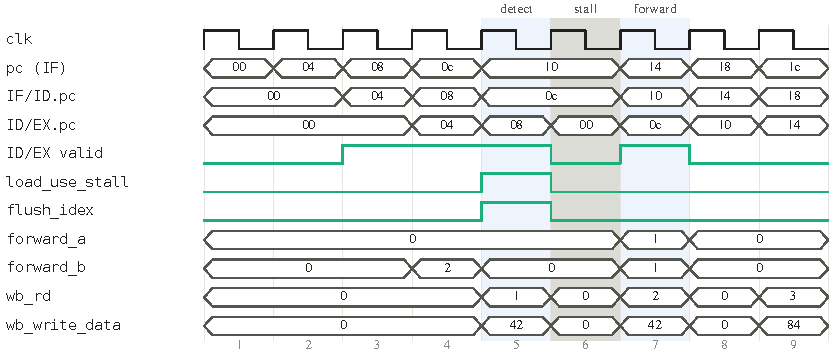
\includegraphics[width=\textwidth]{figures/wave_load_use.pdf}
\caption{Load-use benchmark (\code{addi x1,x0,42}; \code{sw x1,0(x0)}; \code{lw x2,0(x0)}; \code{add x3,x2,x2}), from the simulation dump. In cycle~4 the SW receives its store data from EX/MEM (\code{forward\_b}$=2$). In cycle~5 the LW is in EX and the dependent ADD is in ID, so \code{load\_use\_stall} rises. In cycle~6 the PC and IF/ID hold their values and ID/EX carries a bubble (valid low). In cycle~7 the ADD executes with both operands forwarded from MEM/WB (\code{forward\_a}$=$\code{forward\_b}$=1$), and x3$=84$ is written back in cycle~9.}
\label{fig:wave-lu}
\end{figure*}

\begin{figure*}[t]
\centering
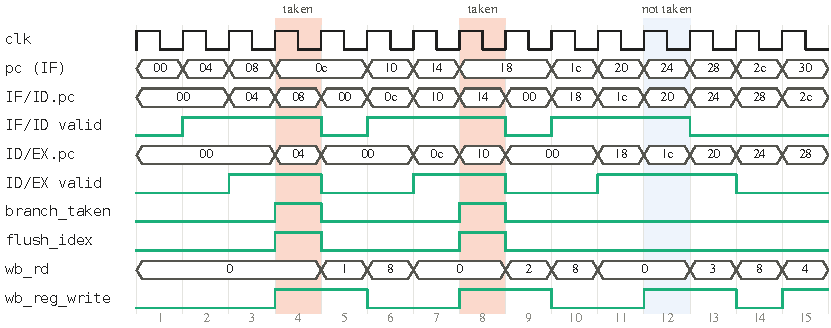
\includegraphics[width=\textwidth]{figures/wave_branches.pdf}
\caption{Branch benchmark from the simulation dump. In cycles~4 and~8 a taken BNE/BEQ in EX raises \code{branch\_taken}. The PC is redirected, IF/ID is cleared (valid low), and ID/EX is flushed. The two wrong-path ADDIs (\code{x5}, \code{x6}$\,\leftarrow 99$) never reach write-back. In cycle~12 the BEQ is not taken and the pipeline continues without loss. For branches, \code{wb\_rd} shows instruction bits 11:7 (the value~8), but \code{wb\_reg\_write} is low, so nothing is written. The reset-time NOP (\code{addi x0,x0,0}) asserts RegWrite with $rd=$ x0, which the register file ignores.}
\label{fig:wave-br}
\end{figure*}

\begin{figure}[t]
\centering
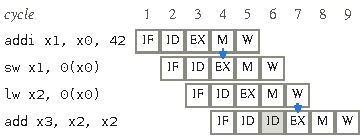
\includegraphics[scale=0.8]{figures/occ_load_use.pdf}\\[4pt]
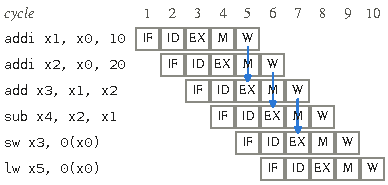
\includegraphics[scale=0.8]{figures/occ_dependent.pdf}\\[4pt]
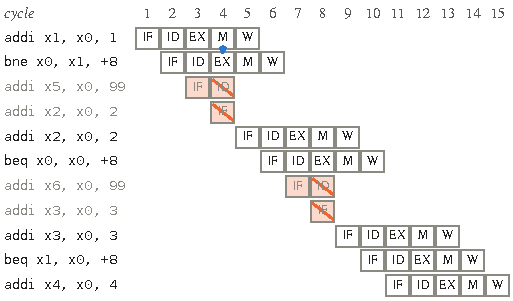
\includegraphics[scale=0.8]{figures/occ_branches.pdf}
\caption{Stage occupancy per cycle, reconstructed from the simulation dump, for the load-use (top), dependent (middle) and branch (bottom) benchmarks. M = MEM and W = WB. Blue arrows show forwarding within a cycle, from the producer's MEM or WB slot to the consumer's EX slot. Grey cells are stall cycles, and orange crossed cells are instructions flushed by a taken branch. The instruction at the branch target is fetched once on the wrong path and once more after the redirect.}
\label{fig:occ}
\end{figure}

\subsection{Not covered}
The following are not tested in the integrated core: illegal instructions (covered at unit level only); misaligned or out-of-range accesses (covered in the memory unit benches only); PC running past the end of instruction memory; reset released exactly on a clock edge; and long or random programs compared against a reference model. No functional-coverage, formal, gate-level or timing simulation was performed.

%% ============================================================================
\section{Performance Analysis}
\label{sec:perf}

\subsection{Method}
Cycles are counted from the first fetch of a non-NOP instruction to the write-back of the last valid instruction. Instructions are counted when they retire from MEM/WB. Then
\[
\text{CPI} = \frac{\text{cycles}}{\text{retired}}, \qquad \text{IPC} = \frac{1}{\text{CPI}}.
\]
The integration testbench writes the counters to a CSV file, and a Python script validates them and computes CPI and IPC. Five benchmarks are short programs that each target one behaviour. The sixth is a straight-line stream of 64 independent ADDIs, which shows how the fixed fill cost is spread over a longer program.

\begin{table}[t]
\centering
\caption{Measured performance (Verilator 5.054)}
\label{tab:perf}
\footnotesize
\setlength{\tabcolsep}{4pt}
\begin{tabular}{@{}lrrrrrr@{}}
\toprule
Benchmark & Cycles & Instr. & Stalls & Taken & CPI & IPC \\
\midrule
Independent & 9  & 5 & 0 & 0 & 1.800 & 0.556 \\
Dependent   & 10 & 6 & 0 & 0 & 1.667 & 0.600 \\
Load-use    & 9  & 4 & 1 & 0 & 2.250 & 0.444 \\
Branches    & 15 & 7 & 0 & 2 & 2.143 & 0.467 \\
Three ADDI  & 7  & 3 & 0 & 0 & 2.333 & 0.429 \\
Long arith.\ & 68 & 64 & 0 & 0 & 1.063 & 0.941 \\
\bottomrule
\end{tabular}
\end{table}

\subsection{Results and cycle model}
Table~\ref{tab:perf} gives the measured counts. Every row satisfies
\begin{equation}
\text{cycles} = N + 4 + S + 2B_{\text{taken}},
\label{eq:cycles}
\end{equation}
where $N$ is the number of retired instructions, $S$ is the number of load-use stall cycles and $B_{\text{taken}}$ is the number of taken branches. The constant~4 is the pipeline fill: the first instruction needs five cycles to reach write-back, and each later one adds one cycle. The \emph{Dependent} program has six instructions, five of which depend on earlier results, yet it shows zero stalls. Forwarding and the bypass handle every one of those dependencies.

The first five programs are short, so the fill cost dominates and CPI lies between 1.67 and 2.33. The fill is paid only once, however: the 64-instruction stream takes 68 cycles, a CPI of 1.06. In general, from (\ref{eq:cycles}),
\[
\text{CPI} = 1 + \frac{4 + S + 2B_{\text{taken}}}{N} \;\xrightarrow{N\rightarrow\infty}\; 1 + s + 2b,
\]
where $s$ and $b$ are the stall and taken-branch rates per instruction. Fig.~\ref{fig:cpi} shows this convergence. A hazard-free stream approaches CPI~$=1$. With 10\% load-use stalls and 5\% taken branches, CPI settles at 1.2.

\begin{figure}[t]
\centering
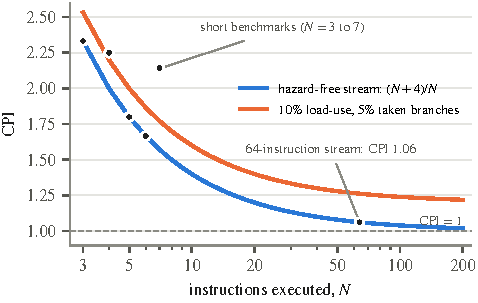
\includegraphics[width=\columnwidth]{figures/cpi_vs_n.pdf}
\caption{CPI against program length from (\ref{eq:cycles}). The dots are the six measured benchmarks. Each one matches (\ref{eq:cycles}) exactly for its own stall and branch counts. Note the logarithmic $x$ axis.}
\label{fig:cpi}
\end{figure}

\subsection{Comparison with alternative designs}
\label{sec:perf-cmp}
The as-built RTL has no switch to disable forwarding, so the alternatives are evaluated with an issue-timing model (\code{scripts/model.py}). The model executes each benchmark in a small instruction-set simulator to obtain the dynamic instruction stream and branch outcomes. It then computes the cycle in which each instruction can enter ID under a given hazard policy. Run with the as-built policy, the model reproduces all six measured cycle and stall counts exactly, and the two alternatives change only the policy:
\begin{itemize}
  \item \emph{No forwarding}: the same pipeline with only the WB$\rightarrow$ID bypass. A consumer waits in ID until its producer reaches WB, so distance-1 and distance-2 dependencies cost two and one stall cycles.
  \item \emph{Stall on every branch}: fetch stops after every branch until it resolves, so not-taken branches also cost two cycles.
\end{itemize}

\begin{figure}[t]
\centering
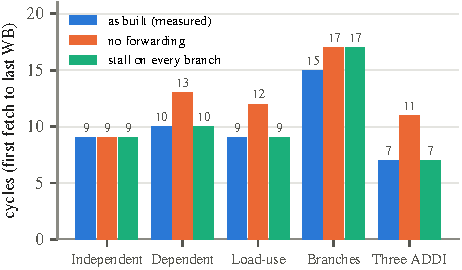
\includegraphics[width=\columnwidth]{figures/policy_cycles.pdf}
\caption{Cycles per benchmark: as built (measured) and the two alternative hazard policies (model validated against the measured counters). The 64-instruction stream is omitted for scale; it takes 68 cycles under all three policies.}
\label{fig:policy}
\end{figure}

\begin{table}[t]
\centering
\caption{Cycles and CPI under alternative hazard policies}
\label{tab:policy}
\footnotesize
\setlength{\tabcolsep}{3.6pt}
\begin{tabular}{@{}lrrrrrr@{}}
\toprule
 & \multicolumn{2}{c}{As built} & \multicolumn{2}{c}{No forwarding} & \multicolumn{2}{c}{Stall on branch} \\
\cmidrule(lr){2-3}\cmidrule(lr){4-5}\cmidrule(l){6-7}
Benchmark & Cyc. & CPI & Cyc. & CPI & Cyc. & CPI \\
\midrule
Independent & 9  & 1.80 & 9  & 1.80 & 9  & 1.80 \\
Dependent   & 10 & 1.67 & 13 & 2.17 & 10 & 1.67 \\
Load-use    & 9  & 2.25 & 12 & 3.00 & 9  & 2.25 \\
Branches    & 15 & 2.14 & 17 & 2.43 & 17 & 2.43 \\
Three ADDI  & 7  & 2.33 & 11 & 3.67 & 7  & 2.33 \\
Long arith.\ & 68 & 1.06 & 68 & 1.06 & 68 & 1.06 \\
\bottomrule
\end{tabular}
\end{table}

Fig.~\ref{fig:policy} and Table~\ref{tab:policy} show the result. Forwarding removes 23\% of the cycles on \emph{Dependent}, 25\% on \emph{Load-use} and 36\% on \emph{Three ADDI}, where every instruction depends on the one before it. On \emph{Independent} and \emph{Long arithmetic}, which have no dependencies, it has no effect, as expected. Predict-not-taken saves 2 of 17 cycles on \emph{Branches}, because one of its three branches falls through.

\textbf{Single-cycle baseline.} A single-cycle core with the same functional units would execute $N$ instructions in $N$ cycles (CPI~$=1$), but at a longer period $T_{\text{sc}}$. The pipelined core takes $N\cdot\text{CPI}_{\text{p}}$ cycles at period $T_{\text{p}}$. The pipeline is faster whenever
\[
\frac{T_{\text{sc}}}{T_{\text{p}}} > \text{CPI}_{\text{p}}.
\]
With five roughly balanced stages, $T_{\text{sc}}/T_{\text{p}}$ approaches 5, minus pipeline-register overhead~\cite{hennessy-quant}. On our short benchmarks the pipeline wins once that ratio exceeds 1.67--2.33. For long programs it wins once the ratio exceeds $1+s+2b$. Because neither design's period was measured (Section~\ref{sec:synth}), we state this as a break-even condition rather than a speed-up figure. No single-cycle version of this core exists in the repository. Its components were, however, verified individually before integration.

%% ============================================================================
\section{Synthesis}
\label{sec:synth}

\begin{table}[t]
\centering
\caption{Yosys \code{synth\_xilinx} resource estimate (7-series)}
\label{tab:synth}
\footnotesize
\begin{tabular}{@{}lrL{4.1cm}@{}}
\toprule
Resource & Count & Breakdown / use \\
\midrule
LUTs & 469 & LUT2 56, LUT3 133, LUT4 123, LUT5 118, LUT6 39 \\
Flip-flops & 349 & FDRE 314, FDCE 32 (PC), FDSE 3 \\
CARRY4 & 36 & ALU, PC$+4$, branch-target adders \\
MUXF7 / MUXF8 & 9 / 3 & wide multiplexers \\
RAM32M & 12 & register file (distributed RAM) \\
RAMB18E1 & 1 & data memory (block RAM) \\
\midrule
Max.\ frequency & -- & \textbf{not measured} \\
\bottomrule
\end{tabular}
\end{table}

\code{riscv\_top} has only \code{clk} and \code{rst\_n} as ports. Since no logic drives an output, any synthesis tool (Yosys or Vivado) correctly removes the entire core as dead logic. To obtain meaningful numbers, we synthesised a scratch copy of the RTL in which the PC and the write-back port (\code{rd}, data, enable) are exposed as outputs. In that copy, the instruction word is supplied from an input port, so that the tool cannot constant-fold the program ROM. The shared RTL was not modified. Table~\ref{tab:synth} lists the result for a Xilinx 7-series target~\cite{ug474}. The register file maps to 12 RAM32M distributed-RAM primitives. The data memory maps to a block RAM, whose read address can be taken from the EX/MEM pipeline register.

These are \emph{pre-place-and-route} estimates from Yosys. We did not run Vivado implementation or deploy to an FPGA, so \textbf{we report no maximum frequency}. By inspection, the longest register-to-register path is probably MEM/WB $\rightarrow$ forwarding multiplexer $\rightarrow$ ALU subtract $\rightarrow$ zero detect $\rightarrow$ branch-taken $\rightarrow$ PC and IF/ID flush. This is a qualitative expectation, not a timing result. Obtaining Fmax requires synthesising the same output-exposing wrapper in Vivado, constraining the clock, running implementation and reading the worst negative slack. We list this as the first item of future work.

%% ============================================================================
\section{Discussion and Limitations}
\label{sec:disc}

\textbf{Conservative SW stall.} SW waits one cycle when its store data comes from the immediately preceding load. Forwarding from MEM/WB into the MEM stage would remove that stall. The current behaviour is correct, and the corner-case bench pins it (exactly five stalls), so any future change will be noticed.

\textbf{Scope.} This is a seven-instruction teaching core. It has no exceptions, interrupts, CSRs, byte or halfword accesses, or jumps. The performance figures describe six straight-line programs. They show how hazards cost cycles, but they are not a general benchmark result.

\textbf{Repository hygiene.} \code{rtl/stages/*.sv} is not part of the build. \code{testbench/pipeline\_tb.sv} is an empty stub, and \code{verification/reference\_model.py} is empty. These are documented in \code{docs/verification.md} for the owners to resolve.

%% ============================================================================
\section{Conclusion and Future Work}
We built a five-stage pipelined RV32I-subset processor in modular SystemVerilog and verified it at three levels: unit benches, integration benches with cycle-level invariant checks, and mutation testing. Its measured cycle counts follow $N+4+S+2B_{\text{taken}}$ exactly, so every cycle beyond the pipeline fill is accounted for by a specific stall or branch. Forwarding and the WB$\rightarrow$ID bypass let fully dependent code run without stalls. Compared with a stall-only design, they save up to 36\% of cycles on our benchmarks.

Future work, in order of priority:
\begin{enumerate}
  \item measure Fmax through Vivado implementation, and deploy the core to an FPGA board;
  \item add a branch predictor (for example a 2-bit BHT with a target buffer), so that taken loop branches stop costing two cycles;
  \item complete the Python reference model, and compare long random programs against it instruction by instruction;
  \item forward into MEM to remove the SW store-data stall.
\end{enumerate}

%% ============================================================================
\appendices
\section{Reproducing the Results}
From the repository root (Verilator and Yosys required):
\begin{itemize}
  \item \code{make test}: runs all 16 testbenches and writes VCDs and \code{performance.csv};
  \item \code{make run}: runs the integration test and prints CPI/IPC;
  \item \code{sh verification/mutation\_check.sh} (run from \code{riscv-processor/}): mutation results;
  \item \code{python3 docs/report/scripts/model.py} then \code{python3 docs/report/scripts/figures.py}: regenerate every data figure from the simulation output. The occupancy reconstruction asserts that it agrees with the dumped pipeline registers;
  \item \code{tectonic report.tex} (in \code{docs/report}): rebuilds this PDF.
\end{itemize}

\balance
\begin{thebibliography}{9}
\bibitem{patterson-riscv}
D.~A. Patterson and J.~L. Hennessy, \emph{Computer Organization and Design RISC-V Edition: The Hardware/Software Interface}, 2nd~ed. Morgan Kaufmann, 2020.

\bibitem{hennessy-quant}
J.~L. Hennessy and D.~A. Patterson, \emph{Computer Architecture: A Quantitative Approach}, 6th~ed. Morgan Kaufmann, 2017.

\bibitem{riscv-spec}
A.~Waterman and K.~Asanovi\'c, Eds., \emph{The RISC-V Instruction Set Manual, Volume~I: Unprivileged ISA}. RISC-V International, 2019.

\bibitem{verilator}
W.~Snyder \emph{et al.}, ``Verilator,'' \url{https://verilator.org}.

\bibitem{yosys}
C.~Wolf, ``Yosys Open SYnthesis Suite,'' \url{https://yosyshq.net/yosys/}.

\bibitem{ug474}
Xilinx, \emph{7 Series FPGAs Configurable Logic Block User Guide}, UG474.

\bibitem{demillo-mutation}
R.~A. DeMillo, R.~J. Lipton, and F.~G. Sayward, ``Hints on test data selection: Help for the practicing programmer,'' \emph{Computer}, vol.~11, no.~4, pp.~34--41, 1978.
\end{thebibliography}

\end{document}
